% SPDX-FileCopyrightText: 2025 Jorge Teixeira Crespo <jorge.teixeira@udc.es>
%
% SPDX-License-Identifier: GPL-2.0-or-later

\chapter{Implementation}
\label{chap:implementation}

\lettrine{T}{he} deployment of the new infrastructure begins with provisioning a dedicated physical server hosted at Hetzner\cite{hetzner-server-bidding}. This server replaces the previous GPUL machines (\texttt{gpulino} and \texttt{gpulon}), and is named \texttt{gpulux}, reflecting its role as the unified and modernized core system.

\section{Installation and Base System}

The base system was installed using Hetzner's \texttt{installimage}\cite{hetzner-installimage} provisioning tool. The configuration focused on separating system and data storage for flexibility and performance.

Debian was chosen as the operating system, a decision rooted in its renowned stability for server roles, as well as the board's deep familiarity with the distribution. This choice also honors GPUL's historical ties to Debian and the contributions of past board members who are official Debian maintainers\cite{berto-debian-page}.

\subsection*{installimage Configuration}

The installation was performed on the two 512 GB disks using software RAID 1 to ensure redundancy. The two 2 TB disks were left untouched during provisioning and later configured manually.

The following snippet shows the \texttt{installimage} configuration file:

\begin{lstlisting}[language=bash,caption={Hetzner's installimage script for automated Debian installation on gpulux.}]
## ====================
##  HARD DISK DRIVE(S):
## ====================

DRIVE1 /dev/nvme2n1
DRIVE2 /dev/nvme3n1

## ===============
##  SOFTWARE RAID:
## ===============

SWRAID 1
SWRAIDLEVEL 1

## ==========
##  HOSTNAME:
## ==========

HOSTNAME gpulux

## =============
##  MISC CONFIG:
## =============

USE_KERNEL_MODE_SETTING yes

## ==========================
##  PARTITIONS / FILESYSTEMS:
## ==========================

PART swap  swap   32G
PART /boot ext3  1024M
PART /     ext4   all

## ========================
##  OPERATING SYSTEM IMAGE:
## ========================

IMAGE /root/.oldroot/nfs/install/../images/Debian-1208-bookworm-amd64-base.tar.gz
\end{lstlisting}

This setup results in the following RAID arrays:

\begin{itemize}
  \item \texttt{/dev/md0} - 32 GB swap
  \item \texttt{/dev/md1} - 1 GB \texttt{/boot}
  \item \texttt{/dev/md2} - remaining space (440 GB) for root filesystem
\end{itemize}

\subsection*{Post-Install Configuration}

After installation, the two 2 TB NVMe drives (\texttt{/dev/nvme0n1} and \texttt{/dev/nvme1n1}) were manually configured into a new RAID 1 array, \texttt{/dev/md3}. For security hardening, SSH access for the \texttt{root} user was disabled, and a new admin user, \texttt{tei*****}, was created with \texttt{sudo} privileges. Access for this user is granted via SSH with public key authentication, as password authentication has been disabled server-wide.

\section{Containerization with Incus}

Incus is not included in the standard Debian 12 (Bookworm) repositories, so it must be installed from the \texttt{bookworm-backports} repository. The backports provide newer software versions that are scheduled for inclusion in future Debian releases, in this case, Debian 13 (Trixie).

To enable the backports, a new APT source file is created, including both the official Debian mirror and the Hetzner mirror for optimized download speeds.

\begin{lstlisting}[language=bash,caption={APT sources list to enable the bookworm-backports repository.}]
deb http://mirror.hetzner.com/debian bookworm-backports main
deb http://deb.debian.org/debian bookworm-backports main
\end{lstlisting}

With the backports repository configured, Incus can be installed. Only the \texttt{incus-base} package is installed, as this provides the necessary tools for managing containers without the overhead of full virtual machine support. This approach aligns with the current plan, and support for VMs can be added later if needed.

\begin{lstlisting}[language=bash,caption={Installing the Incus server from Debian backports.}]
sudo apt update
sudo apt install incus-base/bookworm-backports
\end{lstlisting}

To manage Incus, users must be added to the \texttt{incus-admin} group. The administrative user, \texttt{tei*****}, was added to this group.

\subsection*{Initial Incus Configuration}

Incus was initialized using the \texttt{incus admin init} command. The key configuration choices from the interactive setup are summarized below:
\begin{itemize}
    \item \textbf{Mode:} Standalone (non-clustered).
    \item \textbf{Storage Pool:} A new BTRFS storage pool named \texttt{default} was created on the dedicated data RAID array (\texttt{/dev/md3}).
    \item \textbf{Network:} A new local network bridge, \texttt{incusbr0}, was configured with the IPv4 subnet \texttt{10.42.0.1/24} and NAT enabled. IPv6 was disabled for this bridge.
    \item \textbf{Remote Access:} The Incus server is not exposed over the network.
    \item \textbf{Image Management:} Automatic updates for stale cached images were enabled.
\end{itemize}

\section{Monitoring Stack}

With the Incus environment established, the next step is to create containers to host the various services that will run on the new infrastructure. Each service, or group of related services, is isolated within its own container, providing a clean and manageable separation of concerns.

The first container to be created is for the monitoring stack. This stack is a critical component of the new infrastructure, providing insights into the health and performance of the host system and the services it runs.

\subsection*{Monitoring Container}

A new container named \texttt{monitoring} is launched using the official Debian 12 image. The following command is used:

\begin{lstlisting}[language=bash,caption={Creating the monitoring container with a Debian 12 image.}]
incus launch images:debian/12 monitoring
\end{lstlisting}

Once the container is running, it is possible to get an interactive shell inside it to perform administrative tasks. This is achieved with the \texttt{exec} command:

\begin{lstlisting}[language=bash,caption={Obtaining a shell inside the monitoring container.}]
incus exec monitoring -- bash
\end{lstlisting}

Inside the \texttt{monitoring} container, a full monitoring stack is deployed. This stack consists of three key components:

\begin{itemize}
    \item \textbf{Prometheus:} For collecting and storing time-series data (metrics).
    \item \textbf{Loki:} For collecting and storing logs.
    \item \textbf{Grafana:} For visualizing data from both Prometheus and Loki.
\end{itemize}

\subsection*{Prometheus Configuration}

Prometheus was installed following the official documentation\cite{prometheus-getting-started} and configured to scrape both itself and the Incus host metrics:

\begin{lstlisting}[caption={Prometheus configuration to scrape metrics from itself and the Incus host.}]
scrape_configs:
  - job_name: "prometheus"
    static_configs:
      - targets: ["localhost:9090"]
  - job_name: "incus"
    metrics_path: '/1.0/metrics'
    scheme: 'https'
    tls_config:
      insecure_skip_verify: true
    static_configs:
      - targets: ['10.42.0.1:8444']
\end{lstlisting}

The host was previously configured to expose metrics without authentication using:

\begin{lstlisting}[language=bash]
incus config set core.metrics_address=:8444
incus config set core.metrics_authentication=false
\end{lstlisting}

\subsection*{Loki, Grafana and Journal Logs Collection}

Loki and Grafana were installed in the \texttt{monitoring} container following their official documentation\cite{grafana-install-debian,loki-storage-retention}. Grafana's configuration is managed via its web UI, so it maintains its default settings post-installation.

Loki was configured to store logs on the container's filesystem in the \texttt{/data/loki} directory. A retention period of 744 hours (approximately one month) was set, after which older logs are automatically purged. It was made accessible from the host using a proxy device, which allows requests from the host's loopback interface to reach the Loki instance:

\begin{lstlisting}[language=bash]
incus config device add monitoring loki-proxy proxy \
  listen=tcp:127.0.0.1:3100 connect=tcp:127.0.0.1:3100
\end{lstlisting}

Grafana Alloy, installed on the host\cite{grafana-alloy-install}, forwards logs from the system journal to Loki. The configuration\cite{grafana-alloy-config-example} extracts key metadata such as unit name, boot ID, transport, and priority level:

\begin{lstlisting}[caption={Grafana Alloy configuration for forwarding journal logs to Loki.}]
loki.source.journal "all" {
  relabel_rules = discovery.relabel.journal_relabel.rules
  forward_to    = [loki.write.local.receiver]
}

discovery.relabel "journal_relabel" {
  targets = []

  rule {
    source_labels = ["__journal__systemd_unit"]
    target_label  = "unit"
  }

  rule {
    source_labels = ["__journal__boot_id"]
    target_label  = "boot_id"
  }

  rule {
    source_labels = ["__journal__transport"]
    target_label  = "transport"
  }

  rule {
    source_labels = ["__journal_priority_keyword"]
    target_label  = "level"
  }
}

loki.write "local" {
  endpoint {
    url = "http://127.0.0.1:3100/loki/api/v1/push"
  }
}
\end{lstlisting}

Additionally, Incus is configured to export internal events (e.g., instance start/stop, snapshot creation) directly to Loki\cite{incus-loki-api}:

\begin{lstlisting}[language=bash]
incus config set loki.api.url=http://127.0.0.1:3100
incus config set loki.instance=incus
\end{lstlisting}

\subsection*{Reverse Proxy Setup with Caddy}

To expose web services to the internet, a lightweight container named \texttt{proxy} was created using Alpine Linux. Caddy was installed to act as a reverse proxy. While it will eventually handle all public-facing services, its initial configuration is limited to exposing the Grafana dashboard.

\begin{lstlisting}[language=bash,caption={Commands to set up the Caddy reverse proxy container.}]
incus launch images:alpine/edge proxy
incus exec proxy -- apk add --no-cache caddy
incus file push Caddyfile proxy/etc/caddy/Caddyfile
incus exec proxy -- rc-service caddy start
incus exec proxy -- rc-update add caddy default

incus config device add proxy http80  proxy \
  listen=tcp:0.0.0.0:80  connect=tcp:127.0.0.1:80
incus config device add proxy http443 proxy \
  listen=tcp:0.0.0.0:443 connect=tcp:127.0.0.1:443
\end{lstlisting}

The last two commands add Incus proxy devices\cite{incus-proxy-device} to the \texttt{proxy} container. These devices forward traffic from a public IP address on the host to a port inside the container. Specifically, all traffic arriving at port 80 (HTTP) and 443 (HTTPS) on the host's public network interface is redirected to the corresponding ports on the container's loopback interface, where Caddy is listening.

The Caddyfile used is as follows:

\begin{lstlisting}[caption={Caddyfile configuration to reverse proxy Grafana.}]
grafana.gpulux.org {
  reverse_proxy monitoring:3000
}
\end{lstlisting}

\subsection*{Grafana Usage}

Grafana was accessed using the configured domain. After creating a user, community dashboards for Prometheus and Incus were imported. The Incus dashboard provides a comprehensive overview of the host's performance, displaying real-time metrics such as CPU and memory usage, network traffic, and disk I/O at project and instance level. This allows for quick identification of resource-intensive instances and overall system health monitoring.

The integration with Loki enables deep exploration of system logs. As shown in Figure~\ref{fig:grafana-journal}, logs from the system journal are collected and enriched with metadata labels. This structured logging is invaluable for debugging and security monitoring, allowing for powerful queries and filtering. The figure shows an example of inspecting SSH authentication failure logs, demonstrating how easily security-relevant events can be isolated and analyzed.

\begin{figure}[H]
	\centering
	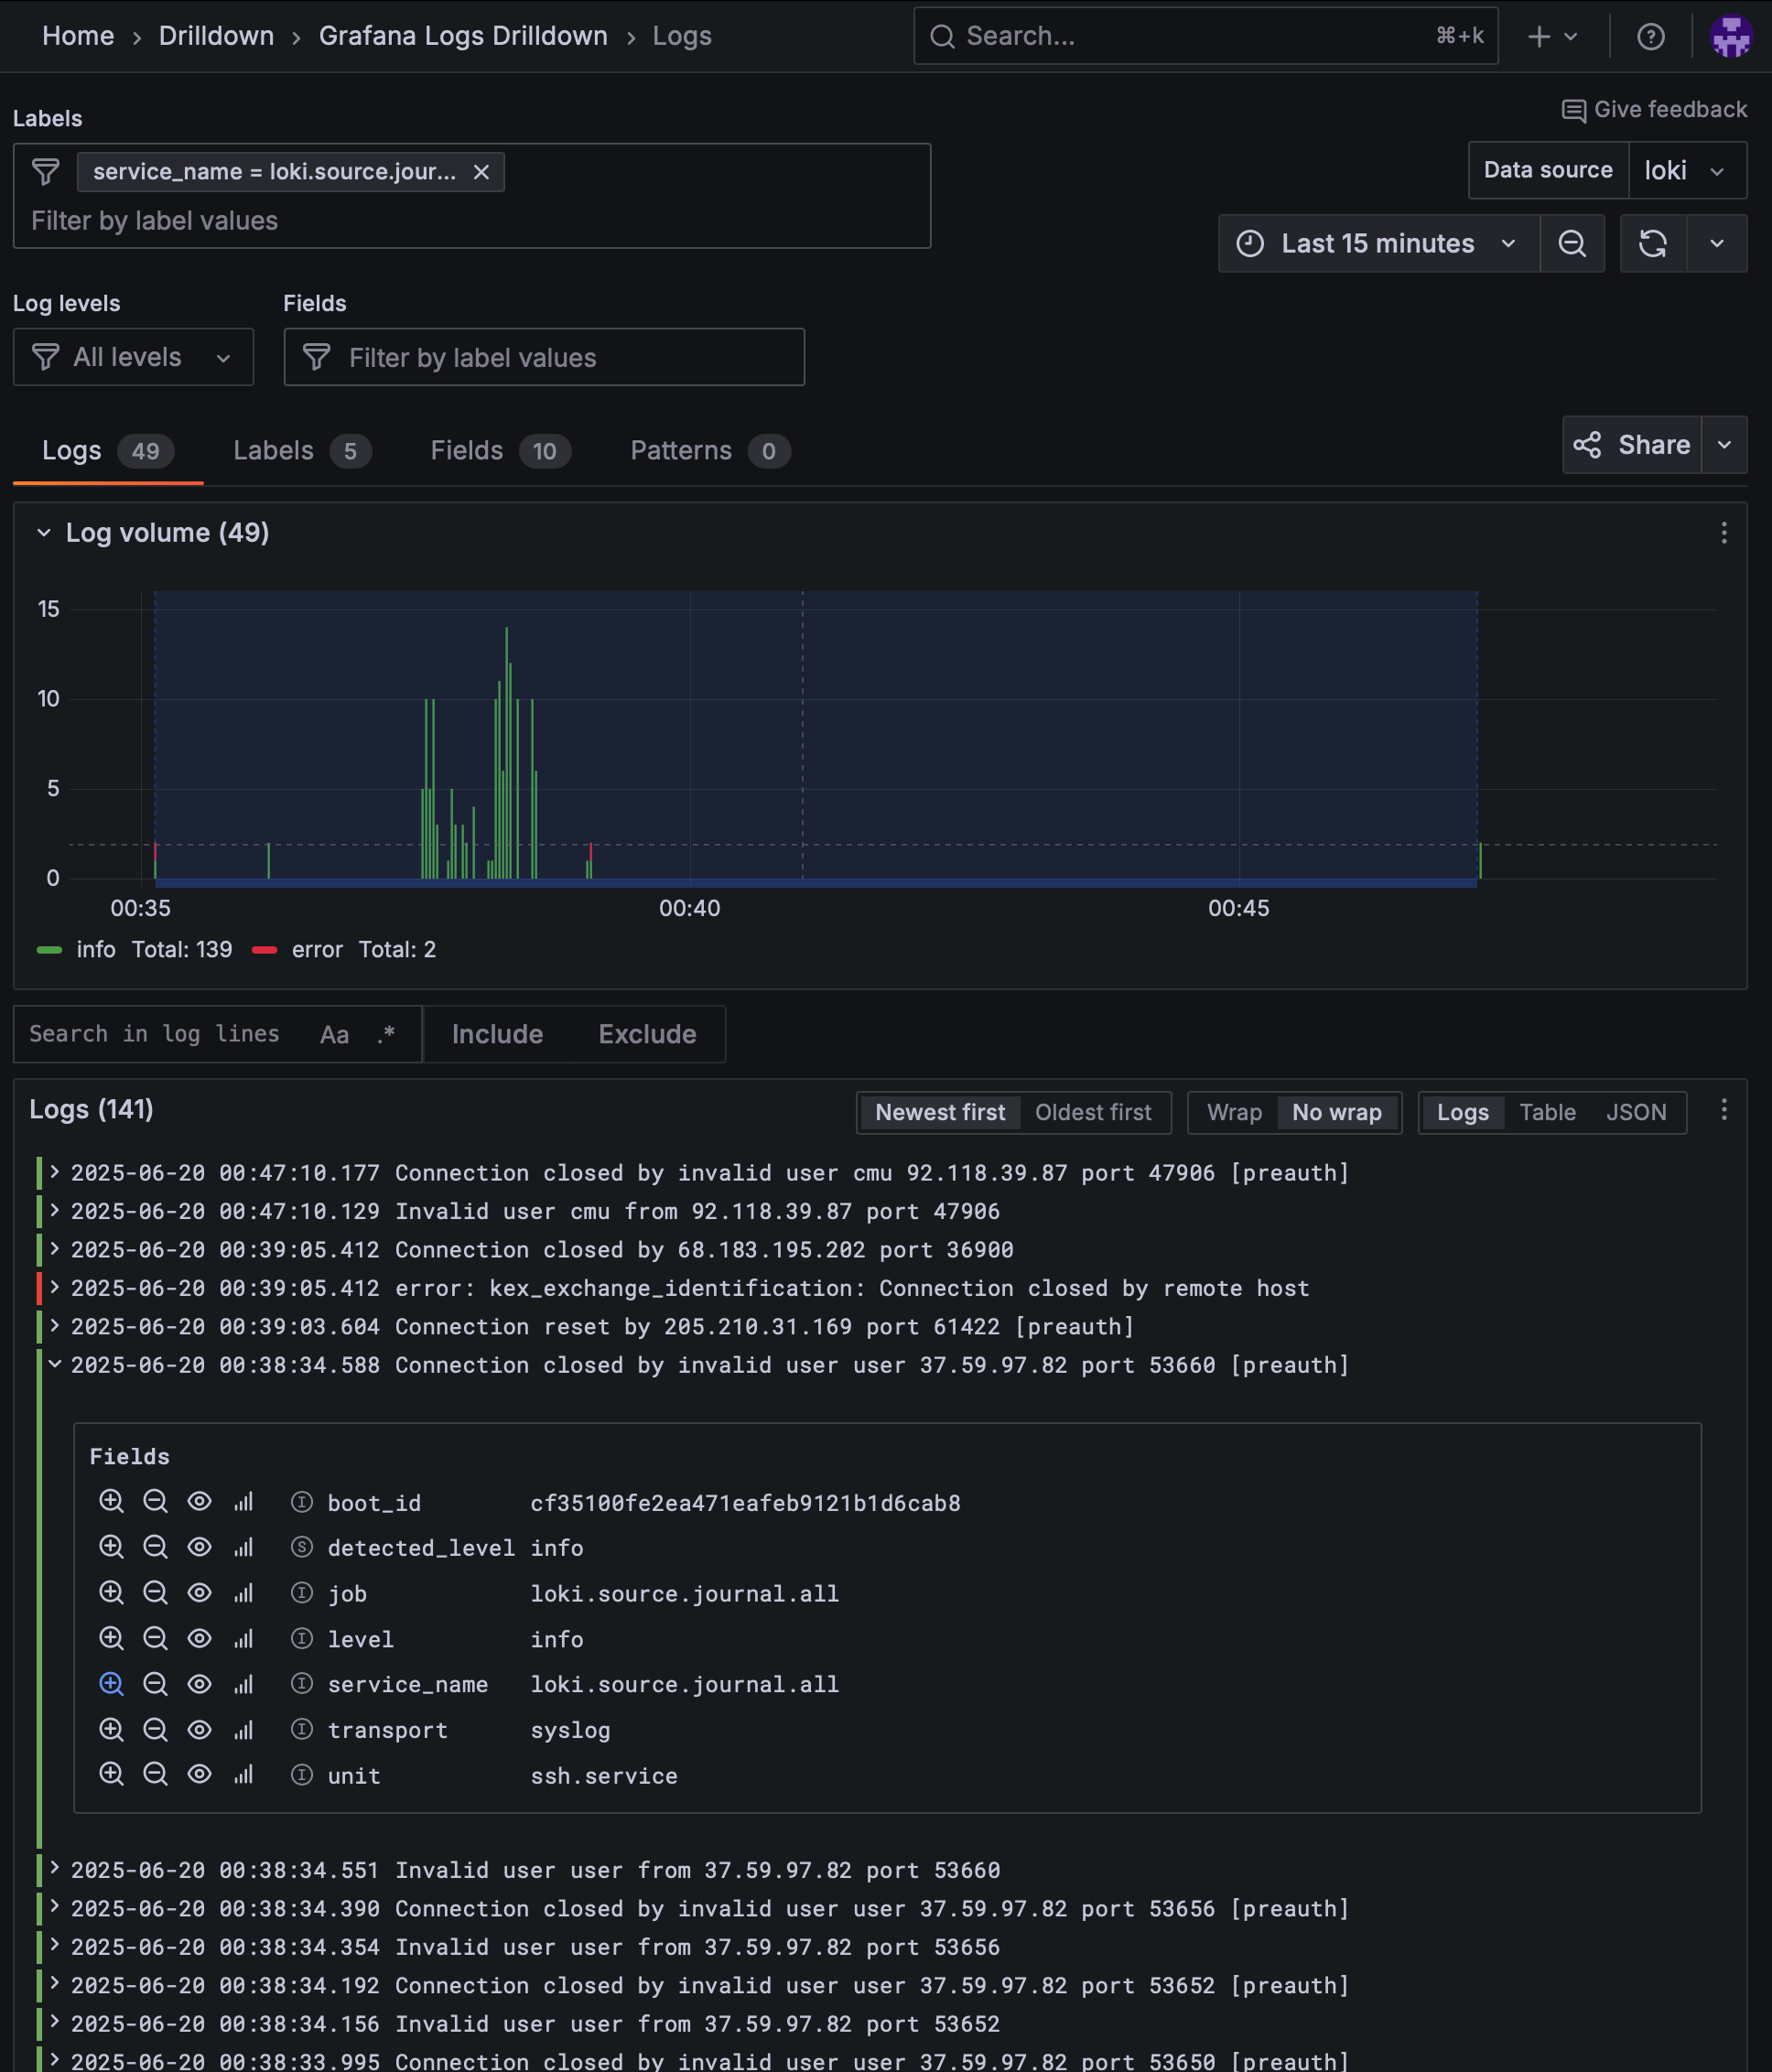
\includegraphics[width=\textwidth]{imaxes/grafana-journal.png}
	\caption{Loki logs in Grafana, showing journal entries with custom labels.}
	\label{fig:grafana-journal}
\end{figure}

\section{Email Server with Mailcow}
\label{sec:mailcow}

Although not discussed in the technology selection chapter, a robust email server is a critical requirement for the new infrastructure, needed for services like Grafana and Passbolt to send alerts and notifications. Mailcow was selected for this role due to its widespread adoption and positive reputation in the open-source self-hosting community. As a complete mail server suite based on Docker, it provides a powerful foundation that will also serve as the Mail Transfer Agent (MTA) for the community's mailing lists, which will be managed by Mailman 3.

\subsection*{Mailcow Container Setup}

To maintain isolation and simplify management, Mailcow is deployed within its own dedicated Incus container. As Mailcow relies on Docker and Docker Compose for its operation, the container needs to be configured to support nested virtualization\cite{incus-faq-docker-nesting}. A new container named \texttt{mailcow} is launched from the Debian 12 image.

\begin{lstlisting}[language=bash,caption={Creating and configuring the Mailcow container.}]
incus launch images:debian/12 mailcow
incus config set mailcow security.nesting=true
incus config set mailcow security.privileged=true
\end{lstlisting}

The \texttt{security.nesting} flag enables the container to run its own containerization environment, while \texttt{security.privileged} is required for Mailcow to manage the networking stack correctly. Inside the container, Docker is installed following the official Docker documentation.

A critical step in deploying an email server on a cloud provider like Hetzner is ensuring that outgoing email ports are not blocked. By default, Hetzner blocks these ports to prevent spam. A support ticket was opened to request the unblocking of these ports for \texttt{gpulux}'s IP address.

To allow external access to Mailcow's services, several ports must be forwarded from the host to the container. This is achieved using Incus proxy devices, which redirect traffic from the host's public IP to the container. Table~\ref{tab:mailcow-ports} lists the required ports.

\begin{table}[H]
    \centering
    \rowcolors{2}{white}{udcgray!25}
    \caption{Ports forwarded to the Mailcow container\cite{mailcow-prerequisites}.}
    \label{tab:mailcow-ports}
    \begin{tabular}{lll}
        \rowcolor{udcpink!25}
        \textbf{Service} & \textbf{Protocol} & \textbf{Port} \\
        \hline
        Postfix SMTP & TCP & 25 \\
        Postfix SMTPS & TCP & 465 \\
        Postfix Submission & TCP & 587 \\
        Dovecot IMAP & TCP & 143 \\
        Dovecot IMAPS & TCP & 993 \\
        Dovecot POP3 & TCP & 110 \\
        Dovecot POP3S & TCP & 995 \\
        Dovecot ManageSieve & TCP & 4190 \\
    \end{tabular}
\end{table}

The commands to create these proxy devices follow a similar pattern as the Caddy proxy setup, created for each port listed in the table. For example, to forward the SMTP port:

\begin{lstlisting}[language=bash,caption={Example of forwarding a port to the Mailcow container.}]
# SMTP (25)
incus config device add mailcow smtp-proxy proxy listen=tcp:0.0.0.0:25 connect=tcp:127.0.0.1:25
\end{lstlisting}

\subsection*{Mailcow Configuration}

After setting up the container and installing Docker, Mailcow is installed by following its official documentation\cite{mailcow-install}. The primary configuration is managed through the \texttt{mailcow.conf} file. Key settings include configuring the server to run behind a reverse proxy\cite{mailcow-reverse-proxy} and disabling IPv6 support to resolve connectivity issues\cite{mailcow-disable-ipv6}. The mail server is configured to run on \texttt{mail.gpulux.org}.

To integrate with the existing monitoring stack, a Prometheus exporter is added to Mailcow's Docker Compose setup. This allows Prometheus to scrape metrics about the mail server's health and performance. The following service definition was added to \texttt{docker\allowbreak-compose.yml}\cite{mailcow-prometheus-exporter}:

\begin{lstlisting}[caption={Docker Compose service for the Mailcow Prometheus exporter.}]
mailcow-exporter:
  image: ghcr.io/mailcow/prometheus-exporter:2
  ports:
    - "9099:9099"
  environment:
    MAILCOW_EXPORTER_HOST: mail.gpulux.org
    MAILCOW_EXPORTER_API_KEY: redacted
  restart: unless-stopped
\end{lstlisting}

Once Mailcow is running, a single mailbox for \texttt{admin@gpulux.org} is created through its web UI. Aliases for \texttt{grafana@gpulux.org} and \texttt{passbolt@gpulux.org} were configured to deliver mail to this main account. These will be used by the respective services to send email notifications and alerts.

\subsection*{Reverse Proxy Configuration}

To expose Mailcow's web interface and mail autoconfiguration endpoints, the Caddy reverse proxy is configured to forward requests for \texttt{mail.gpulux.org} and its autodiscovery subdomains to the Mailcow container.

\begin{lstlisting}[caption={Caddyfile configuration to reverse proxy Mailcow.}]
mail.gpulux.org autodiscover.mail.gpulux.org autoconfig.mail.gpulux.org {
    reverse_proxy mailcow:80
}
\end{lstlisting}

\section{Password Manager with Passbolt}

The next service to be deployed is Passbolt, the password manager chosen to securely manage credentials for the new infrastructure.

\subsection*{Passbolt Container Setup}

Similar to other services, Passbolt is deployed in a dedicated Incus container named \texttt{passbolt} using a Debian 12 image. No special container configuration was required.

\begin{lstlisting}[language=bash,caption={Creating the Passbolt container.}]
incus launch images:debian/12 passbolt
\end{lstlisting}

\subsection*{Passbolt Configuration}

The installation of Passbolt was performed following the official documentation\cite{passbolt-install-debian}. The process involves adding a dedicated APT repository and installing the \texttt{passbolt-ce-server} package, which triggers a configuration wizard that prompts for database settings.

\begin{lstlisting}[language=bash,caption={Installing Passbolt CE server package.}]
sudo apt install passbolt-ce-server
\end{lstlisting}

Passbolt's package includes Nginx for serving its web interface. However, the existing infrastructure uses a central Caddy instance as a reverse proxy. The automated Nginx setup provided by the Passbolt package was disabled, and manual adjustments were made to its configuration file to ensure compatibility. The key changes involved setting the \texttt{X-Forwarded-Proto} header to ensure that Passbolt generates correct HTTPS URLs when operating behind the proxy.

\begin{lstlisting}[caption={Modified Passbolt Nginx configuration to work behind a reverse proxy.}]
#
#  Passbolt.conf - Nginx configuration file to run the Passbolt software.
#

server {

  listen 80;
  listen [::]:80;

  # Managed by Passbolt
  server_name _;

  set $forwarded_proto $http_x_forwarded_proto; # added this line

  client_body_buffer_size     100K;
  client_header_buffer_size   1K;
  client_max_body_size        5M;

  client_body_timeout   10;
  client_header_timeout 10;
  keepalive_timeout     5 5;
  send_timeout          10;

  root /usr/share/php/passbolt/webroot;
  index index.php;
  error_log /var/log/nginx/passbolt-error.log info;
  access_log /var/log/nginx/passbolt-access.log;

  # Managed by Passbolt
  # include __PASSBOLT_SSL__

  location / {
    try_files $uri $uri/ /index.php?$args;
  }

  location ~ \.php$ {
    try_files                $uri =404;
    include                  fastcgi_params;
    fastcgi_pass             unix:/run/php/php8.2-fpm.sock;
    fastcgi_index            index.php;
    fastcgi_intercept_errors on;
    fastcgi_split_path_info  ^(.+\.php)(.+)$;
    fastcgi_param            SCRIPT_FILENAME $document_root$fastcgi_script_name;
    fastcgi_param            SERVER_NAME $http_host;

    fastcgi_param HTTPS $forwarded_proto; # added this line

    fastcgi_param PHP_VALUE  "upload_max_filesize=5M \n post_max_size=5M";
  }

}
\end{lstlisting}

With the Nginx configuration corrected, accessing \texttt{passbolt.gpulux.org} launches the web-based setup wizard. This final step involves configuring the database connection, generating a GPG key for the server, setting up the SMTP connection to Mailcow, and creating the initial administrator account.

\subsection*{Reverse Proxy Configuration}

To expose Passbolt's web interface, the Caddy reverse proxy is configured to forward requests for \texttt{passbolt.gpulux.org} to the Passbolt container.

\begin{lstlisting}[caption={Caddyfile configuration to reverse proxy Passbolt.}]
passbolt.gpulux.org {
    reverse_proxy passbolt:80
}
\end{lstlisting}

Figure~\ref{fig:passbolt-ui} shows the Passbolt interface after configuration, populated with credentials for other services in the infrastructure.

\begin{figure}[H]
	\centering
	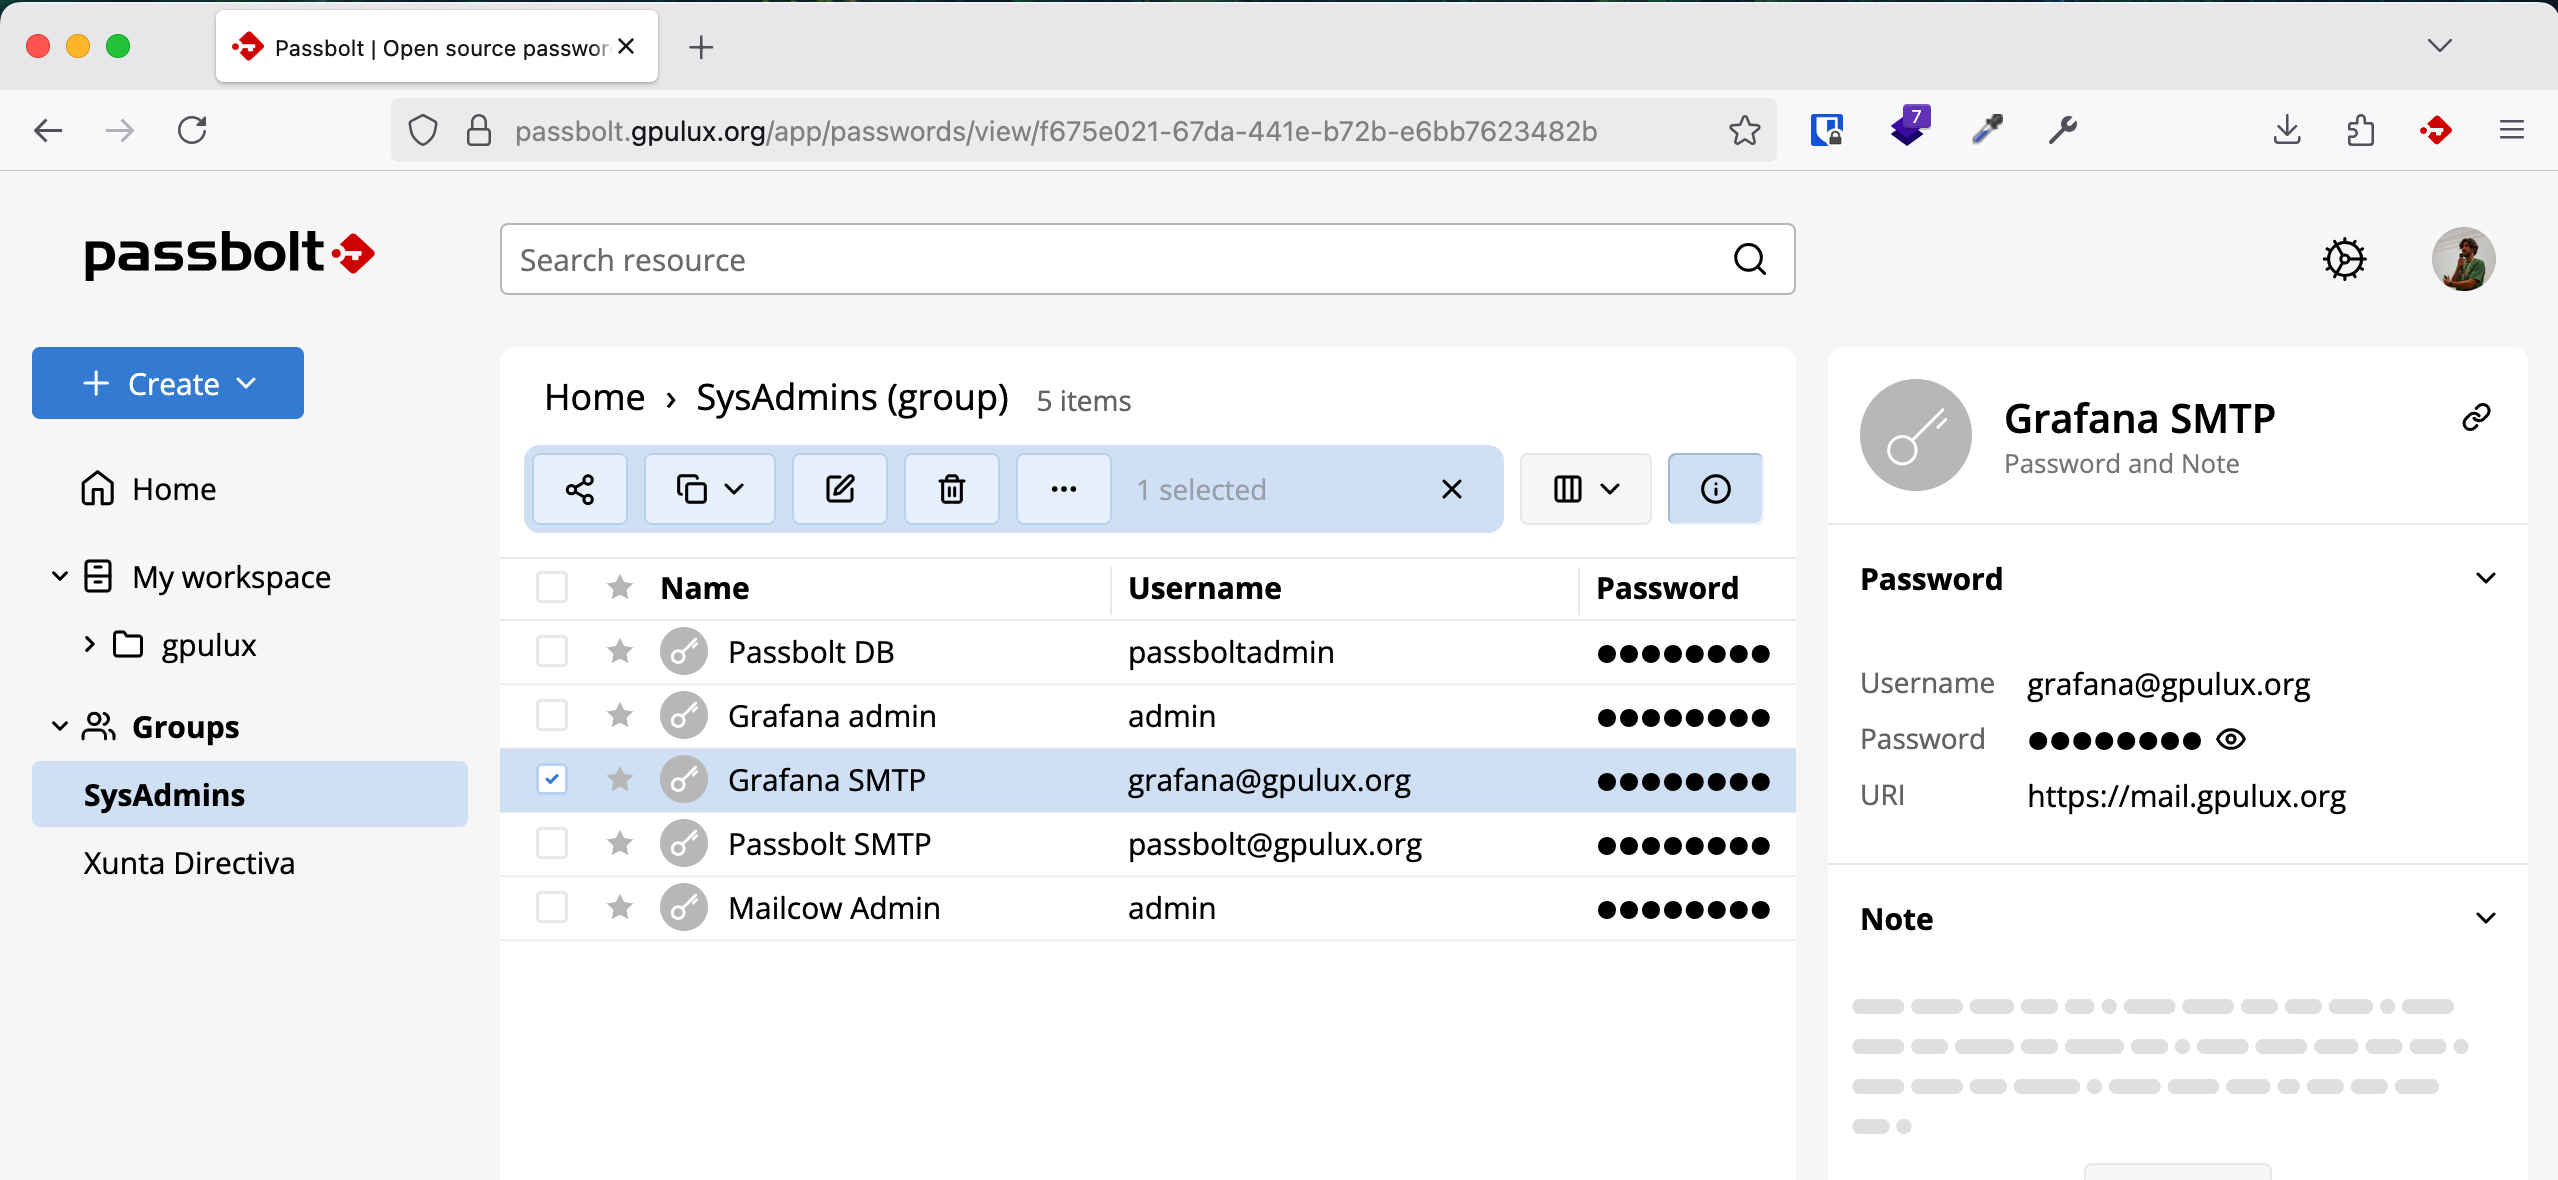
\includegraphics[width=\textwidth]{imaxes/passbolt-gpulux.png}
	\caption{Passbolt web interface showing stored credentials.}
	\label{fig:passbolt-ui}
\end{figure}

\section{Mailing Lists with Mailman 3}
\label{sec:mailman}

With the core services in place, the next step is to deploy the mailing list manager. Mailman 3 was chosen to replace the outdated Mailman 2.1 instance. The order of installation for this service is not critical, as it only depends on previously configured components like the email server.

\subsection*{Mailman Container Setup}

A dedicated Incus container named \texttt{mailman} was created for this service using a Debian 12 image. The setup largely follows the official installation guides:
\begin{itemize}
    \item The official Debian installation guides for Mailman 3:
    \begin{itemize}
        \item \texttt{/usr/share/doc/mailman3/README.Debian}
        \item \texttt{/usr/share/doc/mailman3-web/README.Debian.gz}
        \item \texttt{/usr/share/doc/python3-mailman-hyperkitty/README.rst}
    \end{itemize}
    \item The online documentation for Mailman 3\cite{mailman3-docs}.
\end{itemize}

\begin{lstlisting}[language=bash,caption={Creating the Mailman container.}]
incus launch images:debian/12 mailman
\end{lstlisting}

Inside the container, the \texttt{mailman3-full} package was installed from the Debian repositories. This package bundles Mailman Core, the HyperKitty archiver, and Postorius for web-based list management. However, dependencies such as Postfix, Nginx, and Redis must be installed and configured separately to create a fully functional system.

\subsection*{Mailman Configuration}

The default configurations for Redis were sufficient for this deployment. For Nginx, the provided configuration file at \texttt{/etc/mailman3/nginx.conf} was linked to \texttt{/etc/nginx/\allowbreak sites-enabled/}. The \texttt{server\_name} directive was set to \texttt{\_} to accept requests for any hostname, as Caddy handles the public-facing routing.

The most significant configuration was for Postfix. Since both Mailman and Mailcow operate under the same public IP address, they cannot simultaneously listen on the same standard email ports. To resolve this port conflict and to avoid duplicating email server setup (e.g., SPF, DKIM records), Mailman is configured to use Mailcow as a mail relay.

\begin{itemize}
    \item \textbf{Outgoing Mail:} All outgoing emails from Mailman are relayed through the Mailcow container. This is configured in Mailman's Postfix settings by setting \texttt{relayhost = [mailcow]:25}.
    \item \textbf{Incoming Mail:} Incoming mail for mailing lists (e.g., to \texttt{list@lists.gpulux\allowbreak .org}) is first received by Mailcow and then routed to Mailman's Postfix instance via LMTP. A transport map was added in Mailcow's UI to forward all mail for the \texttt{lists.gpulux\allowbreak .org} subdomain to the Mailman container's internal IP address. Mailcow's Postfix was also configured to trust relays from the local network.
\end{itemize}

This setup centralizes mail handling in Mailcow while allowing Mailman to manage the lists.

\subsection*{Data Migration}

The old mailing lists and their archives from the Mailman 2.1 instance were migrated following the official migration guide\cite{mailman3-migration}. The process involved exporting list configurations and archives from the old server and importing them into Mailman 3.

The following commands demonstrate the import process for a single list, \texttt{xunta@lists .gpulux.org}. The list configuration is imported first, followed by the message archive (\texttt{.mbox} file).

\begin{lstlisting}[language=bash,caption={Commands to migrate a Mailman 2.1 list to Mailman 3.}]
# Import list settings and subscribers
mailman --run-as-root import21 xunta@lists.gpulux.org /opt/mailman-data/config.pck

# Import message archive into HyperKitty
mailman-web hyperkitty_import -l xunta@lists.gpulux.org /opt/mailman-data/xunta.mbox

# Update the search index for the imported list
mailman-web update_index_one_list xunta@lists.gpulux.org
\end{lstlisting}

\subsection*{Reverse Proxy Configuration}

To expose Mailman's web interface (Postorius and HyperKitty), the Caddy reverse proxy is configured to forward requests for \texttt{lists.gpulux.org} to the Mailman container.

\begin{lstlisting}[caption={Caddyfile configuration to reverse proxy Mailman 3.}]
lists.gpulux.org {
    reverse_proxy mailman:80
}
\end{lstlisting}

Figure~\ref{fig:mailman-ui} shows the HyperKitty web archiver after the migration, displaying the imported messages from an old mailing list.

\begin{figure}[H]
	\centering
	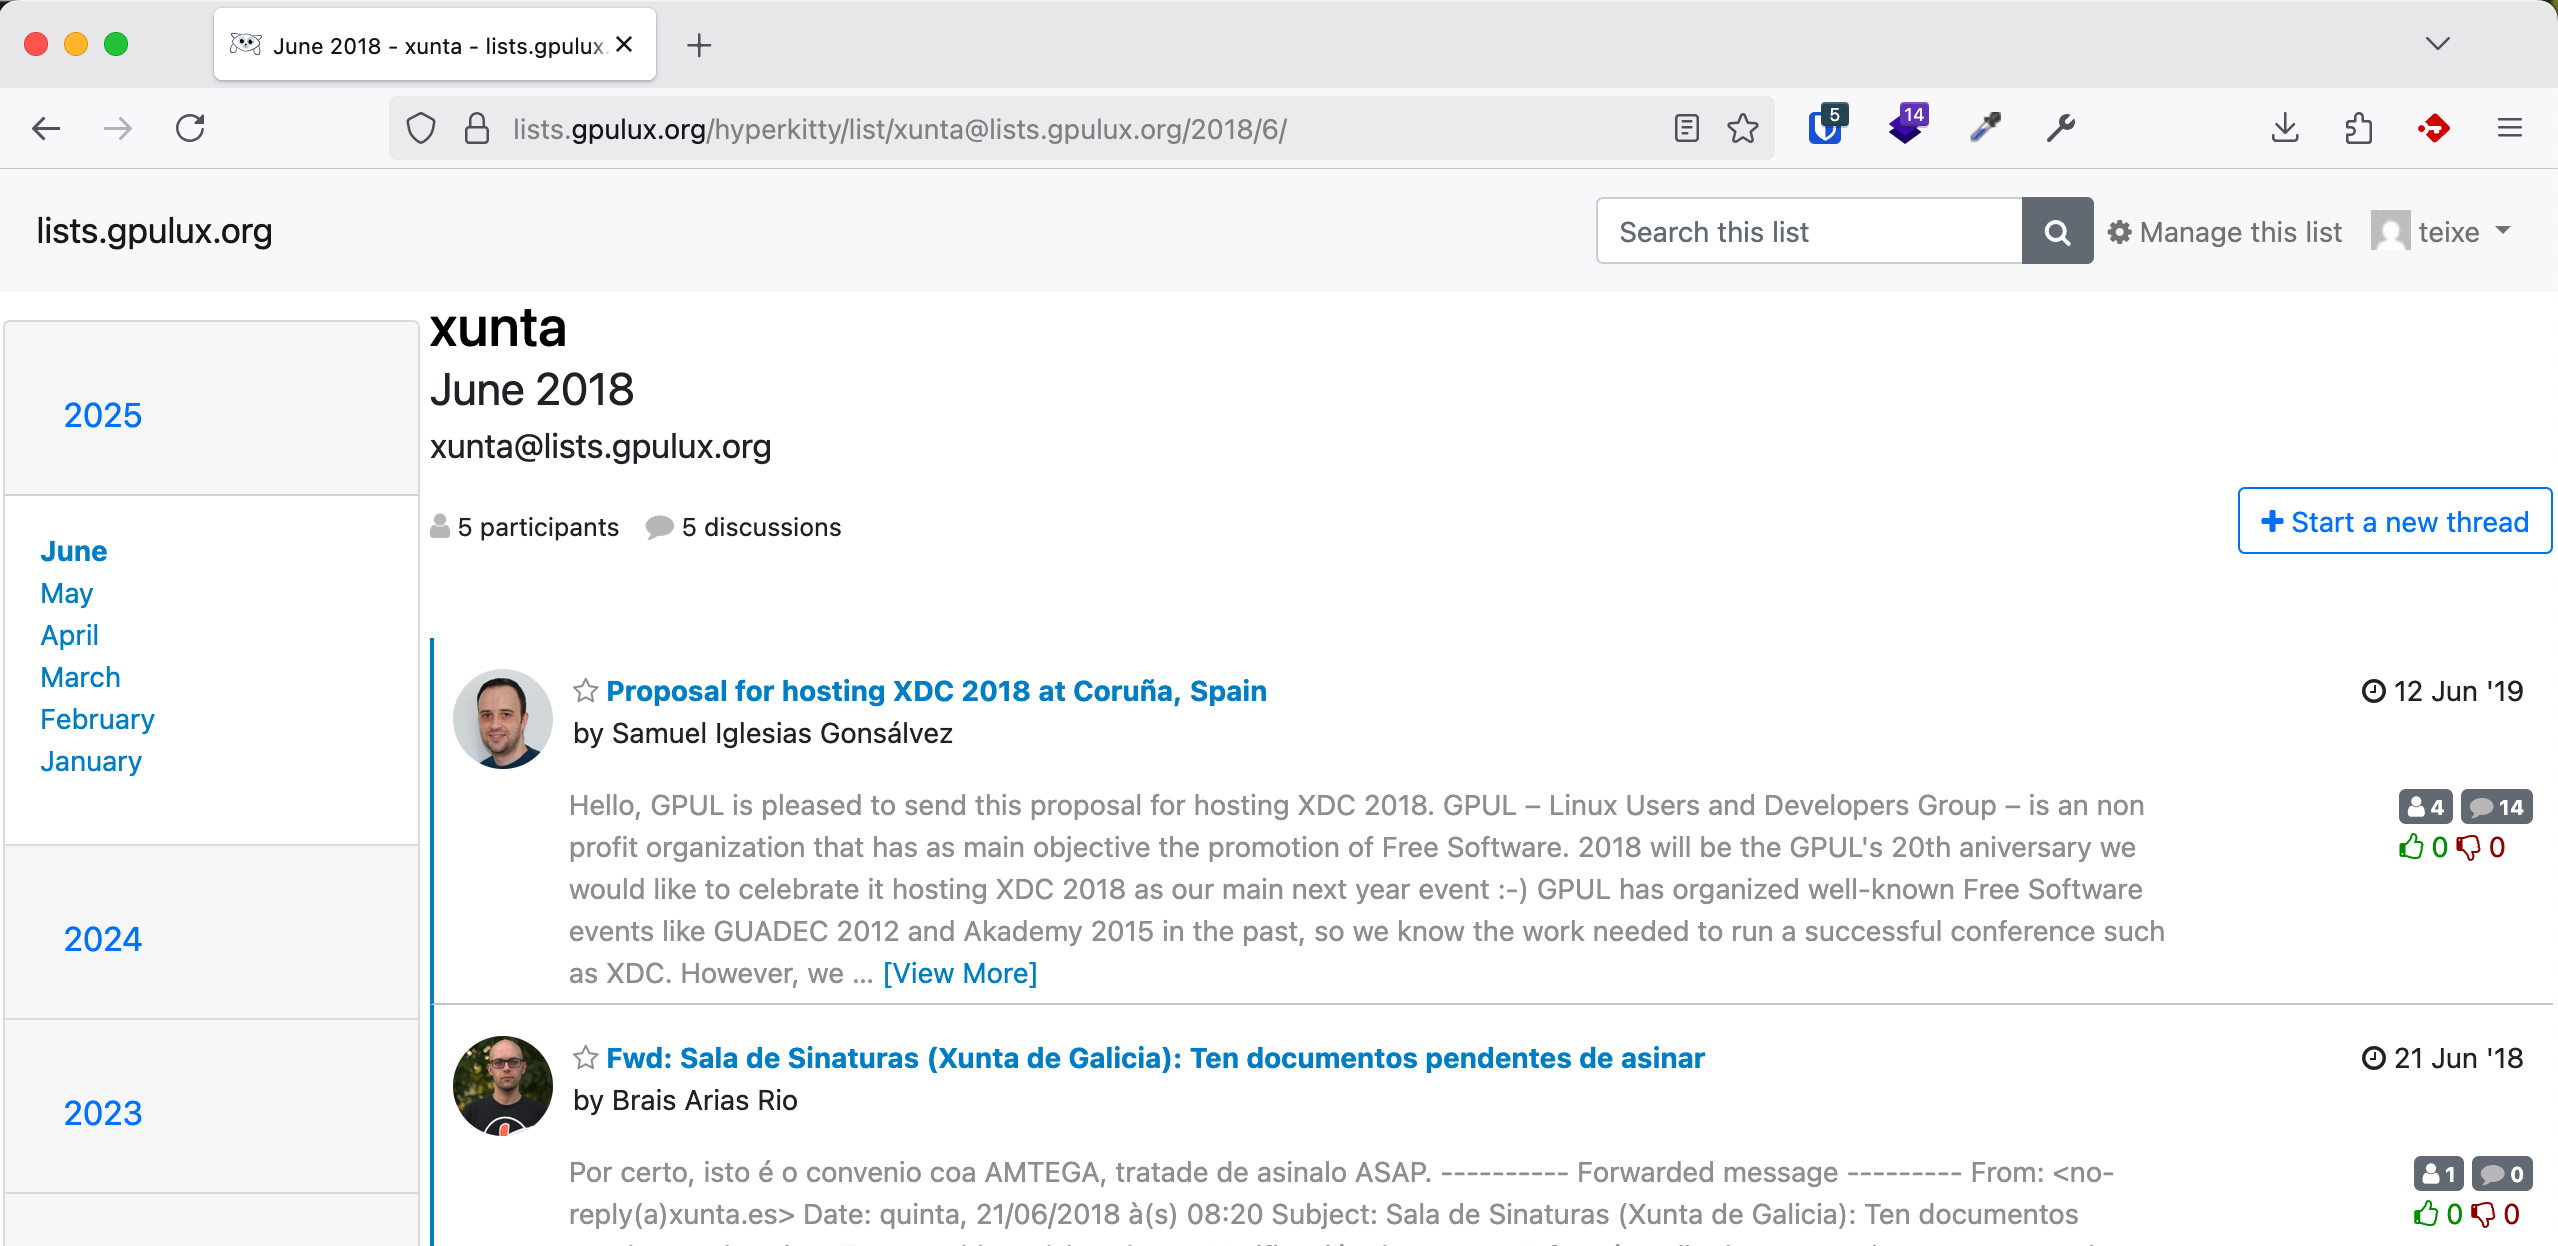
\includegraphics[width=\textwidth]{imaxes/hyperkitty-ui.png}
	\caption{HyperKitty web archiver showing imported mailing list archives.}
	\label{fig:mailman-ui}
\end{figure}

